
\section{视频图像预处理}

\subsection{引言}

本章是视频图像的预处理阶段,首先,获取视频图像;然后对视频图像序列中的每帧图像进行图像预处理。如图\ref{fig:手势运动方向检测流程图}所示。
\begin{figure}[H]
  \centering
  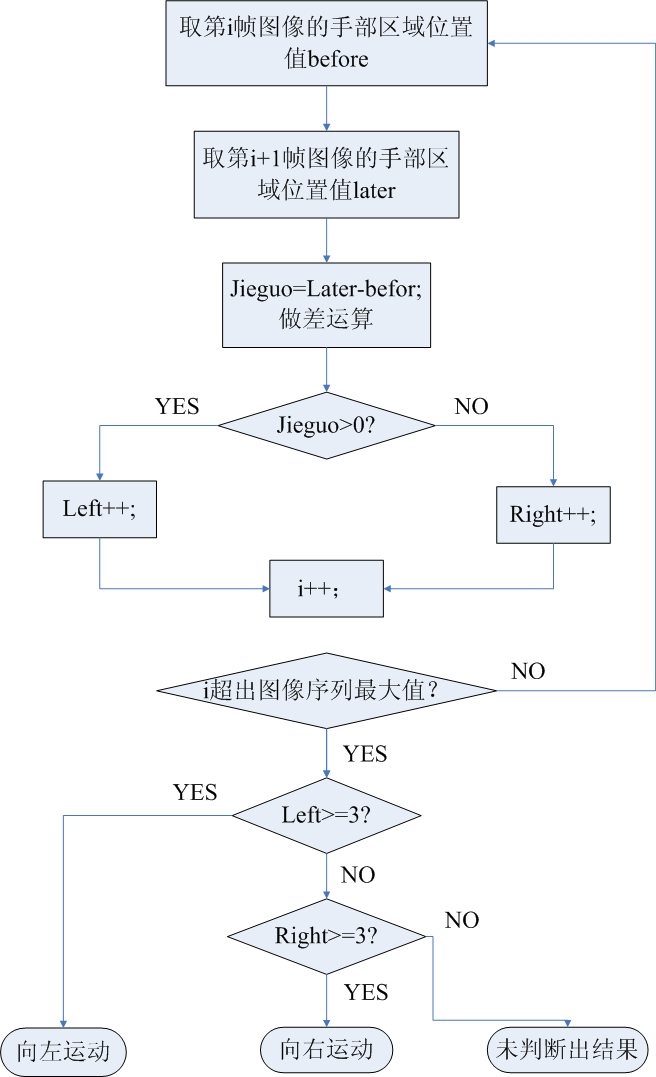
\includegraphics[width=0.5\textwidth]{fig_ch3/手势运动方向检测流程图.png}
  \caption{手势运动方向检测流程图}
  \label{fig:手势运动方向检测流程图}
\end{figure}

由图\ref{fig:手势运动方向检测流程图}可知,视频图像的预处理阶段,首先,获取视频图像;然后对视频图像序列中的每帧图像进行图像预处理。

\subsection{图像的多种显示方式}

分图的情况如图\ref{fig:涂层在冷却过程中残余热应力的变化情况}所示。
\begin{figure}[H]
    \centering
    \begin{minipage}[c]{0.48\textwidth}
        \centering
        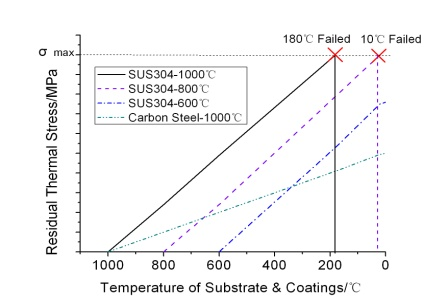
\includegraphics[height=0.2\textheight]{fig_ch3/粗粉_涂层在冷却过程中残余热应力的变化情况.png}
        \subcaption{粗粉涂层}
    \end{minipage}
    \begin{minipage}[c]{0.48\textwidth}
        \centering
        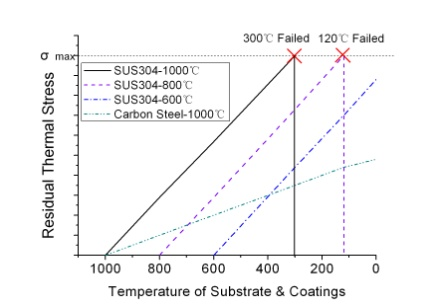
\includegraphics[height=0.2\textheight]{fig_ch3/细粉_涂层在冷却过程中残余热应力的变化情况.png}
        \subcaption{细粉涂层}
    \end{minipage}
    \caption{涂层在冷却过程中残余热应力的变化情况}\label{fig:涂层在冷却过程中残余热应力的变化情况}
\end{figure}

在图中说明比较多的情况下,采取如图\ref{fig:透平膨胀机的组成结构}的格式。
\begin{figure}[H]
  \centering
  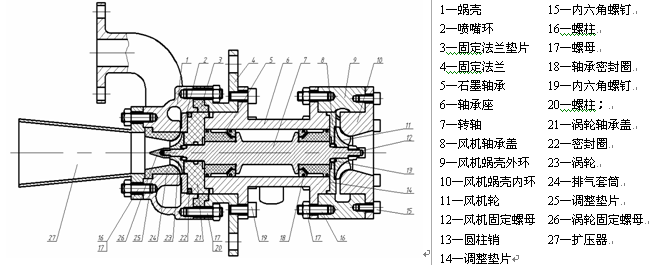
\includegraphics[width=0.7\textwidth]{fig_ch3/透平膨胀机的组成结构.png}
  \caption{透平膨胀机的组成结构}
  \label{fig:透平膨胀机的组成结构}
\end{figure}

\subsection{本章小结}

本章主要介绍了图片的格式。

